\documentclass[10pt]{article}
\usepackage[letterpaper,textwidth=6.75in,top=0.65in,bottom=0.65in]{geometry}
\usepackage{fontspec}
\setmainfont{texgyrepagella}[Extension=.otf,UprightFont=*-regular,BoldFont=*-bold,ItalicFont=*-italic,BoldItalicFont=*-bolditalic]
\setsansfont{texgyreheros}[Extension=.otf,UprightFont=*-regular,BoldFont=*-bold,ItalicFont=*-italic,BoldItalicFont=*-bolditalic]
\usepackage{amsmath,amssymb,booktabs,tabularx,graphicx,xcolor,enumitem}
\usepackage[colorlinks=true,urlcolor=teal,linkcolor=teal]{hyperref}
\usepackage{fancyhdr}
\definecolor{plum}{HTML}{5A405F}
\definecolor{muted}{HTML}{6C6570}
\pagestyle{fancy}\fancyhf{}
\fancyhead[L]{\sffamily\small DeepProbe-VLM / experimental protocol}
\fancyhead[R]{\sffamily\small 7 October 2026}
\fancyfoot[C]{\thepage}
\setlength{\headheight}{14pt}
\setlength{\parindent}{0pt}\setlength{\parskip}{5pt}
\newcolumntype{Y}{>{\raggedright\arraybackslash}X}
\setlist[itemize]{leftmargin=*,nosep,topsep=3pt}
\newcommand{\status}[1]{{\sffamily\color{plum}\small #1}}
\begin{document}
\begin{center}
{\sffamily\LARGE\bfseries DeepProbe-VLM}\par
{\sffamily\large Native-looped video SFT: an executable baseline}\par
\status{PRE-EXPERIMENT RELEASE \quad / \quad NO MEASURED GPU RESULTS}
\end{center}

\textbf{Purpose.} Establish a faithful, reproducible looped vision-language baseline before testing selective visual-state updates and CUDA co-design. This note replaces neither the earlier frozen-model draft nor a finished results paper. It aligns the new figures with the current implementation and separates working software from research hypotheses.

\begin{figure}[h!]
\centering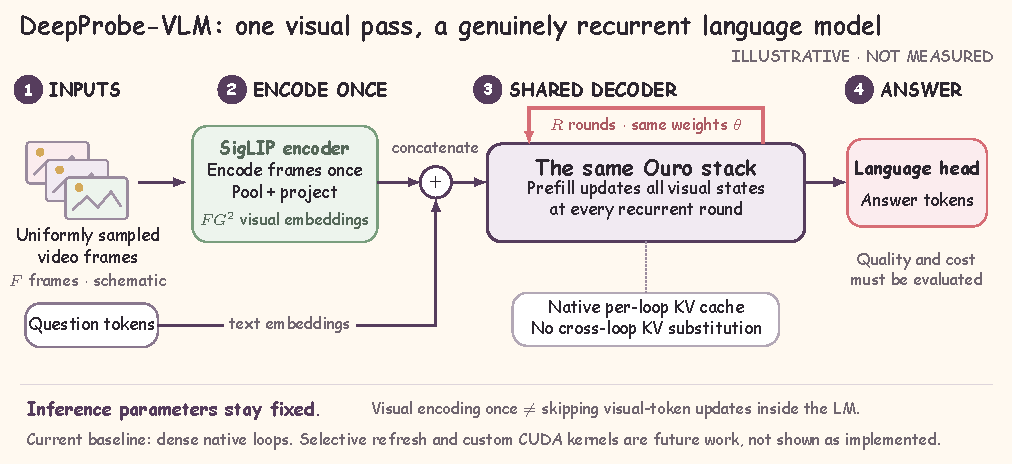
\includegraphics[width=\linewidth]{figures/final/main_overview.pdf}
\caption{One visual encoding pass, followed by a native recurrent language stack. The question bypasses the vision encoder. During prefill, visual states still evolve at every recurrent round. Diagrams are schematic, not measured evidence.}
\end{figure}

\section*{1. What is implemented}
The reference backbone is Ouro-1.4B with its native shared-weight recurrence. SigLIP encodes uniformly sampled frames; a learned spatial pooling/projector produces a bounded visual prefix. An ordinary SmolLM2-1.7B language backbone is also supported as an external comparison. All models are resolved at immutable repository commits.

Training has two stages: projector alignment with frozen backbones, then answer-supervised SFT through the full recurrent language model. The default SFT recipe also unfreezes the vision encoder. The unused adaptive-exit gate stays frozen. This is fixed-depth full-backpropagation SFT, \emph{not} online test-time training or LoRA.

At inference, weights remain fixed. Native caches are distinct across recurrence depths and reused only across generated tokens at their corresponding depth. There is no shallow-to-deep KV substitution, trained halting policy, or custom CUDA/PTX kernel in this release.

\textbf{Release boundary.} Small CPU models test data handling, gradients, checkpoint round trips and cache consistency. No H20/B300 training run, quality improvement, GPU speedup or memory reduction is claimed here.

\clearpage
\section*{2. Mathematical contract}
For frame features $x_{f,p}=E_{\psi}(V_f)_p$, the connector uses a positive learned gate and pools within adaptive spatial bins $\mathcal B_g$:
\begin{align}
w_{f,p} &= \max\{\sigma(a^\top x_{f,p}+b),\epsilon\},\\
\bar x_{f,g} &= \frac{\sum_{p\in\mathcal B_g} w_{f,p}x_{f,p}}
                         {\sum_{p\in\mathcal B_g}w_{f,p}},
&v_{f,g}&=\operatorname{MLP}_{\phi}(\bar x_{f,g}).
\end{align}
With $F$ frames and a $G\times G$ pooling grid, the prefix has $N_v=FG^2$ visual tokens. The starting recipe uses $F=8$, $G=4$, hence 128 visual tokens. This is a low-cost temporal-coverage baseline, not evidence that eight frames preserve all long-video events.

Let $H^{(0)}$ concatenate the visual prefix and prompt embeddings. Schematically, the native backbone performs recurrent updates with shared parameters,
\begin{equation}
H^{(r)}=\mathcal F_{\theta}^{\mathrm{native}}(H^{(r-1)}),
\qquad r=1,\ldots,R.
\end{equation}
This notation summarizes recurrence; the implementation delegates normalization, residual structure and cache indexing to the pinned Ouro code. It does not emulate loops by repeatedly calling a standard language model. Sharing $\theta$ does not imply identical $H^{(r)}$, keys, or values across rounds. Under causal masking, the visual prefix cannot read later question tokens: current visual updates are not query-adaptive.

The supervised objective is final-round, answer-only causal cross-entropy:
\begin{equation}
\mathcal L_{\mathrm{SFT}}=-\frac{1}{|\mathcal A|}
\sum_{t\in\mathcal A}\log p_{\theta,\phi,\psi}
\big(y_t\mid V,q,y_{<t};R\big).
\end{equation}
Prompt, visual-prefix and padding positions are ignored. The wrapper requests final-round logits and computes the shifted loss itself; it does not silently inherit a different weighted-exit objective. Gradients flow through all rounds without inter-round detachment.

\section*{3. What would constitute a research contribution?}
The baseline components above are not claimed as novel. A future contribution must demonstrate a new mechanism and a controlled quality--cost trade-off beyond this dense reference:
\begin{itemize}
\item \textbf{Selective visual-state refresh:} train an internal update policy, preserving a valid dense fallback and cache semantics. Merely selecting frames before the model is a different problem.
\item \textbf{Budget-aware learning:} study an explicit quality--compute objective, then check whether its compute proxy predicts actual latency. No unproved mathematical guarantee is claimed.
\item \textbf{Kernel co-design:} implement compaction, scheduling or fusion only for a mechanism shown useful in profiling; validate both numerical behavior and end-to-end quality.
\end{itemize}
These branches are hypotheses. Sparse masks alone do not show skipped GPU work, and weight sharing alone does not justify cross-round cache reuse.

\clearpage
\section*{4. Training and evaluation protocol}
\begin{figure}[h!]
\centering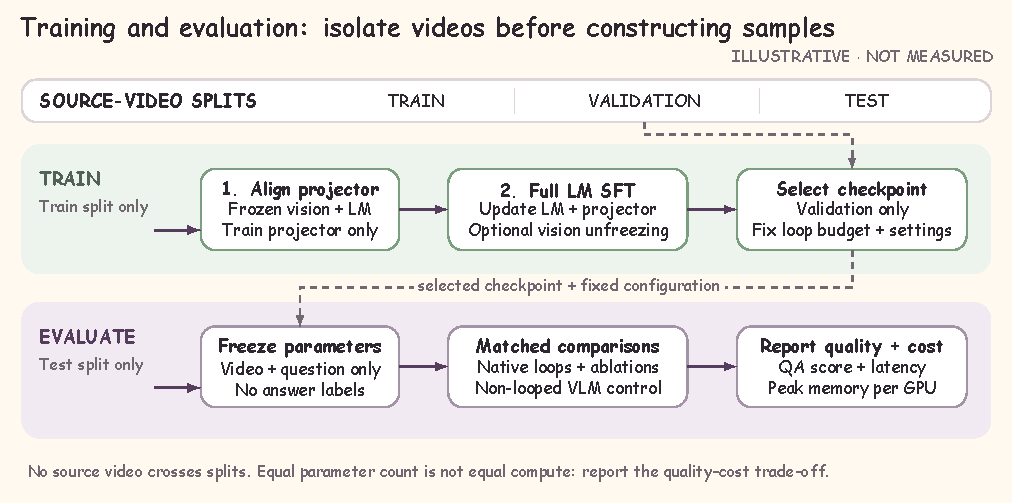
\includegraphics[width=\linewidth]{figures/final/training_protocol.pdf}
\caption{Separate offline optimization and held-out evaluation. Checkpoint provenance carries source-video identities through alignment and SFT. Test questions do not become training examples or checkpoint-selection criteria.}
\end{figure}

\begin{tabularx}{\linewidth}{@{}lYY@{}}\toprule
Resource & Intended role & Required qualification\\\midrule
LLaVA-Video-178K & Training and source-disjoint development split & Start with an explicit subset; preserve upstream media/source identities.\\
Video-MME & Held-out multiple-choice evaluation & Report no-subtitle setting, sample count, and short/medium/long breakdown.\\
MVBench & Held-out task-level evaluation & Respect unavailable/licensed media; label incomplete task coverage as a subset.\\\bottomrule
\end{tabularx}

The manifest records a sample ID, original video ID, relative media path, split, question and target. Clips from the same original video must remain in the same split. The validator detects duplicate normalized IDs and media-source conflicts; it is not a universal content-duplicate detector. Ambiguous upstream IDs require an explicit mapping rather than invented certainty.

The downloader defaults to planning only. It pins repository revisions, estimates transfer size, enforces an explicit size cap and requires opt-in before downloading. Dataset and model licenses remain the user's responsibility; media and weights are not republished in the code repository.

\textbf{Metrics.} Multiple-choice accuracy is separate from normalized exact match for open answers. The latter is not an official semantic judge. For confidence intervals, resample source videos rather than question rows. Paired comparisons must contain identical samples, targets, splits and source identities.

\textbf{Selection.} Select hyperparameters/checkpoints on the development split. Save ancestor training and tuning provenance inside each checkpoint. Final evaluation must reject source overlap with either training or tuning. Missing-media counts and failed examples must be reported, not silently dropped.

\clearpage
\section*{5. H20/B300 execution and measurement}
\begin{figure}[h!]
\centering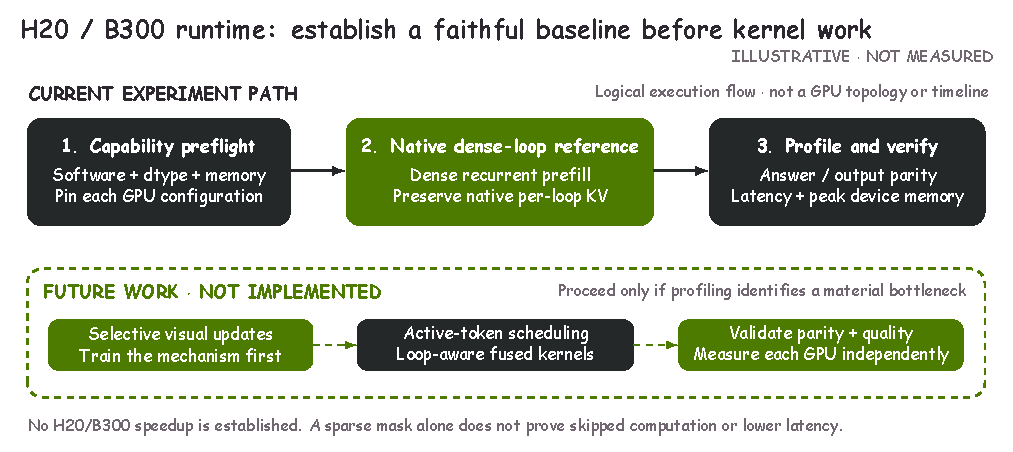
\includegraphics[width=\linewidth]{figures/final/cuda_runtime.pdf}
\caption{White-background, filled green/charcoal runtime diagram. The top row is the current logical execution path; the dashed lower row is future work. This is not a physical GPU topology or measured execution timeline.}
\end{figure}

\textbf{Gate sequence.} Check the actual device, driver and CUDA/PyTorch build. Test a BF16 attention forward and backward pass, then verify an eight-device collective. Run a 20-step model pilot on one GPU and then on eight. Inspect finite loss, all expected gradients, peak memory, checkpoint resume and cached/uncached output parity before committing a large budget.

The included launcher uses ordinary replicated DDP, FP32 trainable weights/Adam state and BF16 autocast. It does not claim FSDP/ZeRO support. Gradient checkpointing reduces activation storage but does not remove recurrent compute. Default full-SFT microbatch is one per device with 16 accumulation steps: global batch 128 on eight GPUs.

\textbf{Timing boundary.} The reference evaluator records preparation, model execution and end-to-end elapsed time, plus peak allocated memory. Model time includes vision encoding, prefill and decode; those components are not separately instrumented yet. Raw timing is cold/mixed and profiler traces add overhead. Neither is a warmed throughput result.

For a publishable systems comparison, use fixed inputs, decoding length, batch, precision and software provenance; add warmup and repeated synchronized measurements. Report median/p95 latency, actual generated tokens, memory and task quality. Measure each GPU family independently. Estimate remaining training time only from observed steady-state step time, adding validation and checkpoint costs.

\clearpage
\section*{6. Minimal ablation matrix}
\begin{tabularx}{\linewidth}{@{}lYY@{}}\toprule
Axis & Controlled comparison & Interpretation\\\midrule
Recurrent depth & Ouro $R=1,2,4$, separately adapted & Quality and cost of native recurrent depth.\\
Ordinary model & SmolLM2, same visual pipeline & External reference; pretraining/size confounds remain.\\
Vision adaptation & Frozen vs trainable encoder & Whether end-to-end visual adaptation matters.\\
Visual budget & $F=4,8,16$; $G=2,4,8$ & Change one axis at a time; temporal vs spatial budget.\\
Alignment & With vs without connector alignment & Include an equal-total-budget comparison.\\
Cache & Cached vs full recomputation & Correctness first; compare same checkpoint/output.\\
Hardware & H20 vs B300 & Matched workload, measured independently.\\\bottomrule
\end{tabularx}

Use seeds 17, 29 and 43 for final model comparisons. An initial pilot is not a multi-seed result. Report both example/step-matched and compute-matched comparisons where feasible: a larger $R$ consumes more computation even at the same parameter count. Changing recurrence depth only at inference is not equivalent to training at that depth.

\textbf{Avoid an invalid claim.} Ouro and SmolLM2 differ in pretraining, tokenizer, parameter count, architecture and initial instruction behavior. A higher benchmark score against that model would be useful evidence, but not causal proof that looping is the sole reason. Count the vision encoder and connector when reporting total VLM parameters.

\section*{7. Reproducibility checklist}
\begin{itemize}
\item Model and dataset commits, manifest hashes, source-disjoint split policy.
\item Training stage, all optimizer/schedule settings, seed, effective global batch and sample budget.
\item Checkpoints with optimizer/RNG state for exact resume; weights-only initialization for stage changes.
\item GPU/driver/CUDA/library versions, actual parameter counts and validation logs.
\item Per-example predictions, strict metric definitions, coverage and source-cluster confidence intervals.
\item No fabricated result tables or forecast improvements presented as observations.
\end{itemize}

\section*{Official implementation and data references}
\small
These are primary resource links for the current baseline, not a complete related-work bibliography. Model commits and data revisions are specified in repository configuration files.
\begin{itemize}
\item \href{https://huggingface.co/ByteDance/Ouro-1.4B}{ByteDance: Ouro-1.4B model and native recurrent implementation}.
\item \href{https://huggingface.co/google/siglip-so400m-patch14-384}{Google: SigLIP SO400M patch14-384}.
\item \href{https://huggingface.co/HuggingFaceTB/SmolLM2-1.7B-Instruct}{Hugging Face: SmolLM2-1.7B-Instruct}.
\item \href{https://huggingface.co/datasets/lmms-lab/LLaVA-Video-178K}{LLaVA-Video-178K dataset}.
\item \href{https://github.com/MME-Benchmarks/Video-MME}{Video-MME official project}; \href{https://github.com/OpenGVLab/Ask-Anything/tree/main/video_chat2}{MVBench / VideoChat2 official project}.
\end{itemize}
\end{document}
